\documentclass{book}
\usepackage[a4paper,
            left=0.5in,
            right=0.5in,
            top=0.5in,
            bottom=0.5in,
            ]{geometry}
\usepackage{minted}
\usepackage{graphicx}
\graphicspath{{.}}
\usepackage{adjustbox}
\usepackage{cprotect}
\setlength{\parindent}{0pt}


\begin{document}
{\Huge \textbf{Title: Basics of Inheritance}}
\\
\par
{\large
\textbf{Objectives: }}
\begin{itemize}
    \item{Understanding parent class and child class (Inheritance)}
    \item{Member access using super keyword}
    \item{Differentiating Overriding and Overloading}
    \item{Experimenting the effect of access specifier in inheritance}
    \item{Final classes and methods}
\end{itemize}
\par
\textbf{Programs:}
\begin{itemize}
    \item{Program to represent Car and Motocycle extending a vehicle class}
    \par
    \begin{center}
    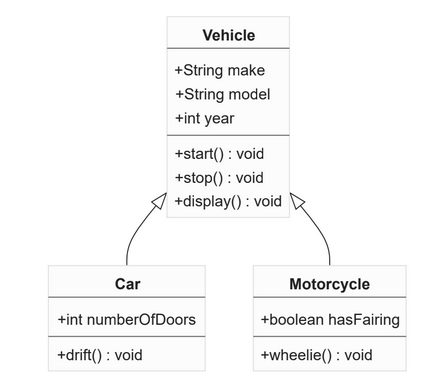
\includegraphics[width=0.5\textwidth,keepaspectratio]{vehicleClassDiagram}
    \end{center}
    \par
    \inputminted{java}{VehicleApp.java}
    \textbf{Output:}
    \input{|"../output.sh VehicleApp"}

    \item{Program to implement SavingAccount and CheckingAccount inherited from generic BankAccount}
    \begin{center}
        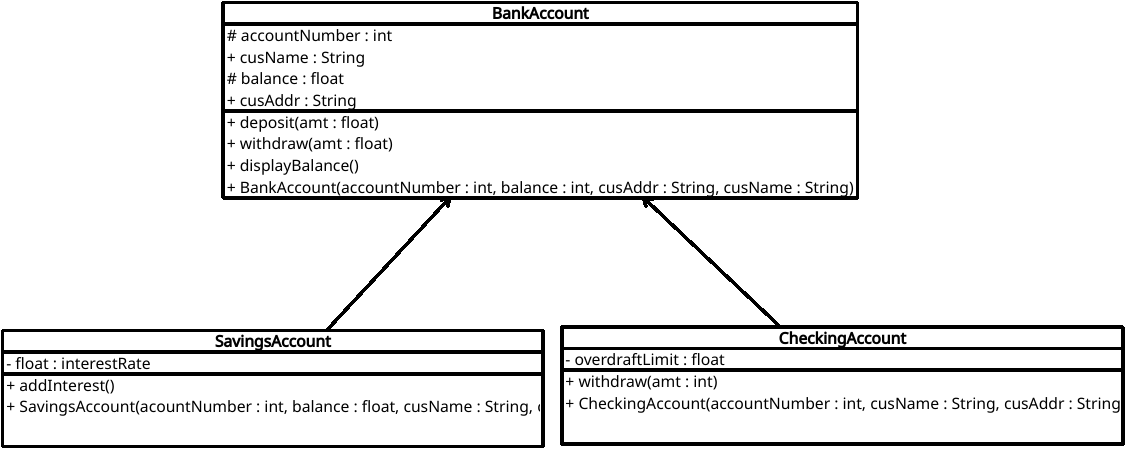
\includegraphics[width=0.8\textwidth,keepaspectratio]{BankClassDiagram}
    \end{center}
    \inputminted{java}{Bank.java}
    \textbf{Output}
    \input{|"../output.sh Bank"}
    \par
    \textbf{Conclusion:} We used inheritance with overriding to implement various methods in a concise way.
\end{itemize}
\end{document}